\section{Timed functions: \textit{libinger}}
\label{sec:libinger}

To address the literature's shortcomings, we have developed
\textit{libinger},\footnote{In the style of GNU's \textit{libiberty}, we named our
system for the command-line switch used to link against it.  As the proverb goes,
``Don't want your function calls to linger?  Link with \texttt{-linger}.''}
a library providing a small API for timed function dispatch
(Listing~\ref{lst:ingerapi}):
\begin{itemize}
\item \texttt{launch()} invokes an ordinary function \texttt{func} with a
time cap of \texttt{time\_us}.  The call to \texttt{launch()} returns when
\texttt{func}
completes, or after approximately \texttt{time\_us} microseconds if \texttt{func} has
not returned
by then.  In the latter case, \textit{libinger} returns an opaque continuation
object recording the execution state.
\item \texttt{resume()} causes a preemptible function to continue after a timeout.
If execution again times out, \texttt{resume()} updates its continuation so the
process may be repeated.  Resuming a function that has already returned has no
effect.
\end{itemize}

\begin{figure}
\begin{lstlisting}[label=lst:ingerapi,caption=Preemptible functions core interface]
struct linger_t {
	bool is_complete;
	cont_t continuation;
};

linger_t launch(Function func,
                  u64 time_us,
                  void *args);
void resume(linger_t *cont, u64 time_us);
\end{lstlisting}
\begin{lstlisting}[label=lst:use, caption=Preemptible function usage example]
linger = launch(task, TIMEOUT, NULL);
if (!linger.is_complete) {
	// Save @linger to a task queue to
	// resume later
	task_queue.push(linger);
}

// Handle other tasks
...
// Resume @task at some later point
linger = task_queue.pop();
resume(&linger, TIMEOUT);
\end{lstlisting}
\end{figure}

Listing~\ref{lst:use} shows an example use of \textit{libinger}
in a task queue manager designed to prevent latency-critical tasks from blocking
behind longer-running
ones. The caller invokes a task with a timeout. If the task does not complete
within the allotted time, the caller saves its continuation in the task queue,
handles other tasks, and later resumes the first task.

In accordance with our goal of language agnosticism, \textit{libinger} exposes both C
and Rust~\cite{www-rustlang} APIs.  To demonstrate the flexibility and composability
of the preemptible function abstraction, we have also created \textit{libturquoise},
a preemptive userland thread library for Rust, by porting an existing futures-based
thread
pool to \textit{libinger}.  We discuss this system in \Chap~\ref{sec:libturquoise}.

Figure~\ref{fig:architecture} shows a dependency graph of the software components
comprising the preemptible functions stack.  The \textit{libinger} library itself is
implemented in approximately 2,500 lines of Rust.  To support calls to nonreentrant
functions, it depends on another library, \textit{libgotcha}, which consists of
another 3,000 lines of C, Rust, and x86-64 assembly.  We cover the details in
\Chap~\ref{sec:libgotcha}.

\begin{figure}
\begin{center}
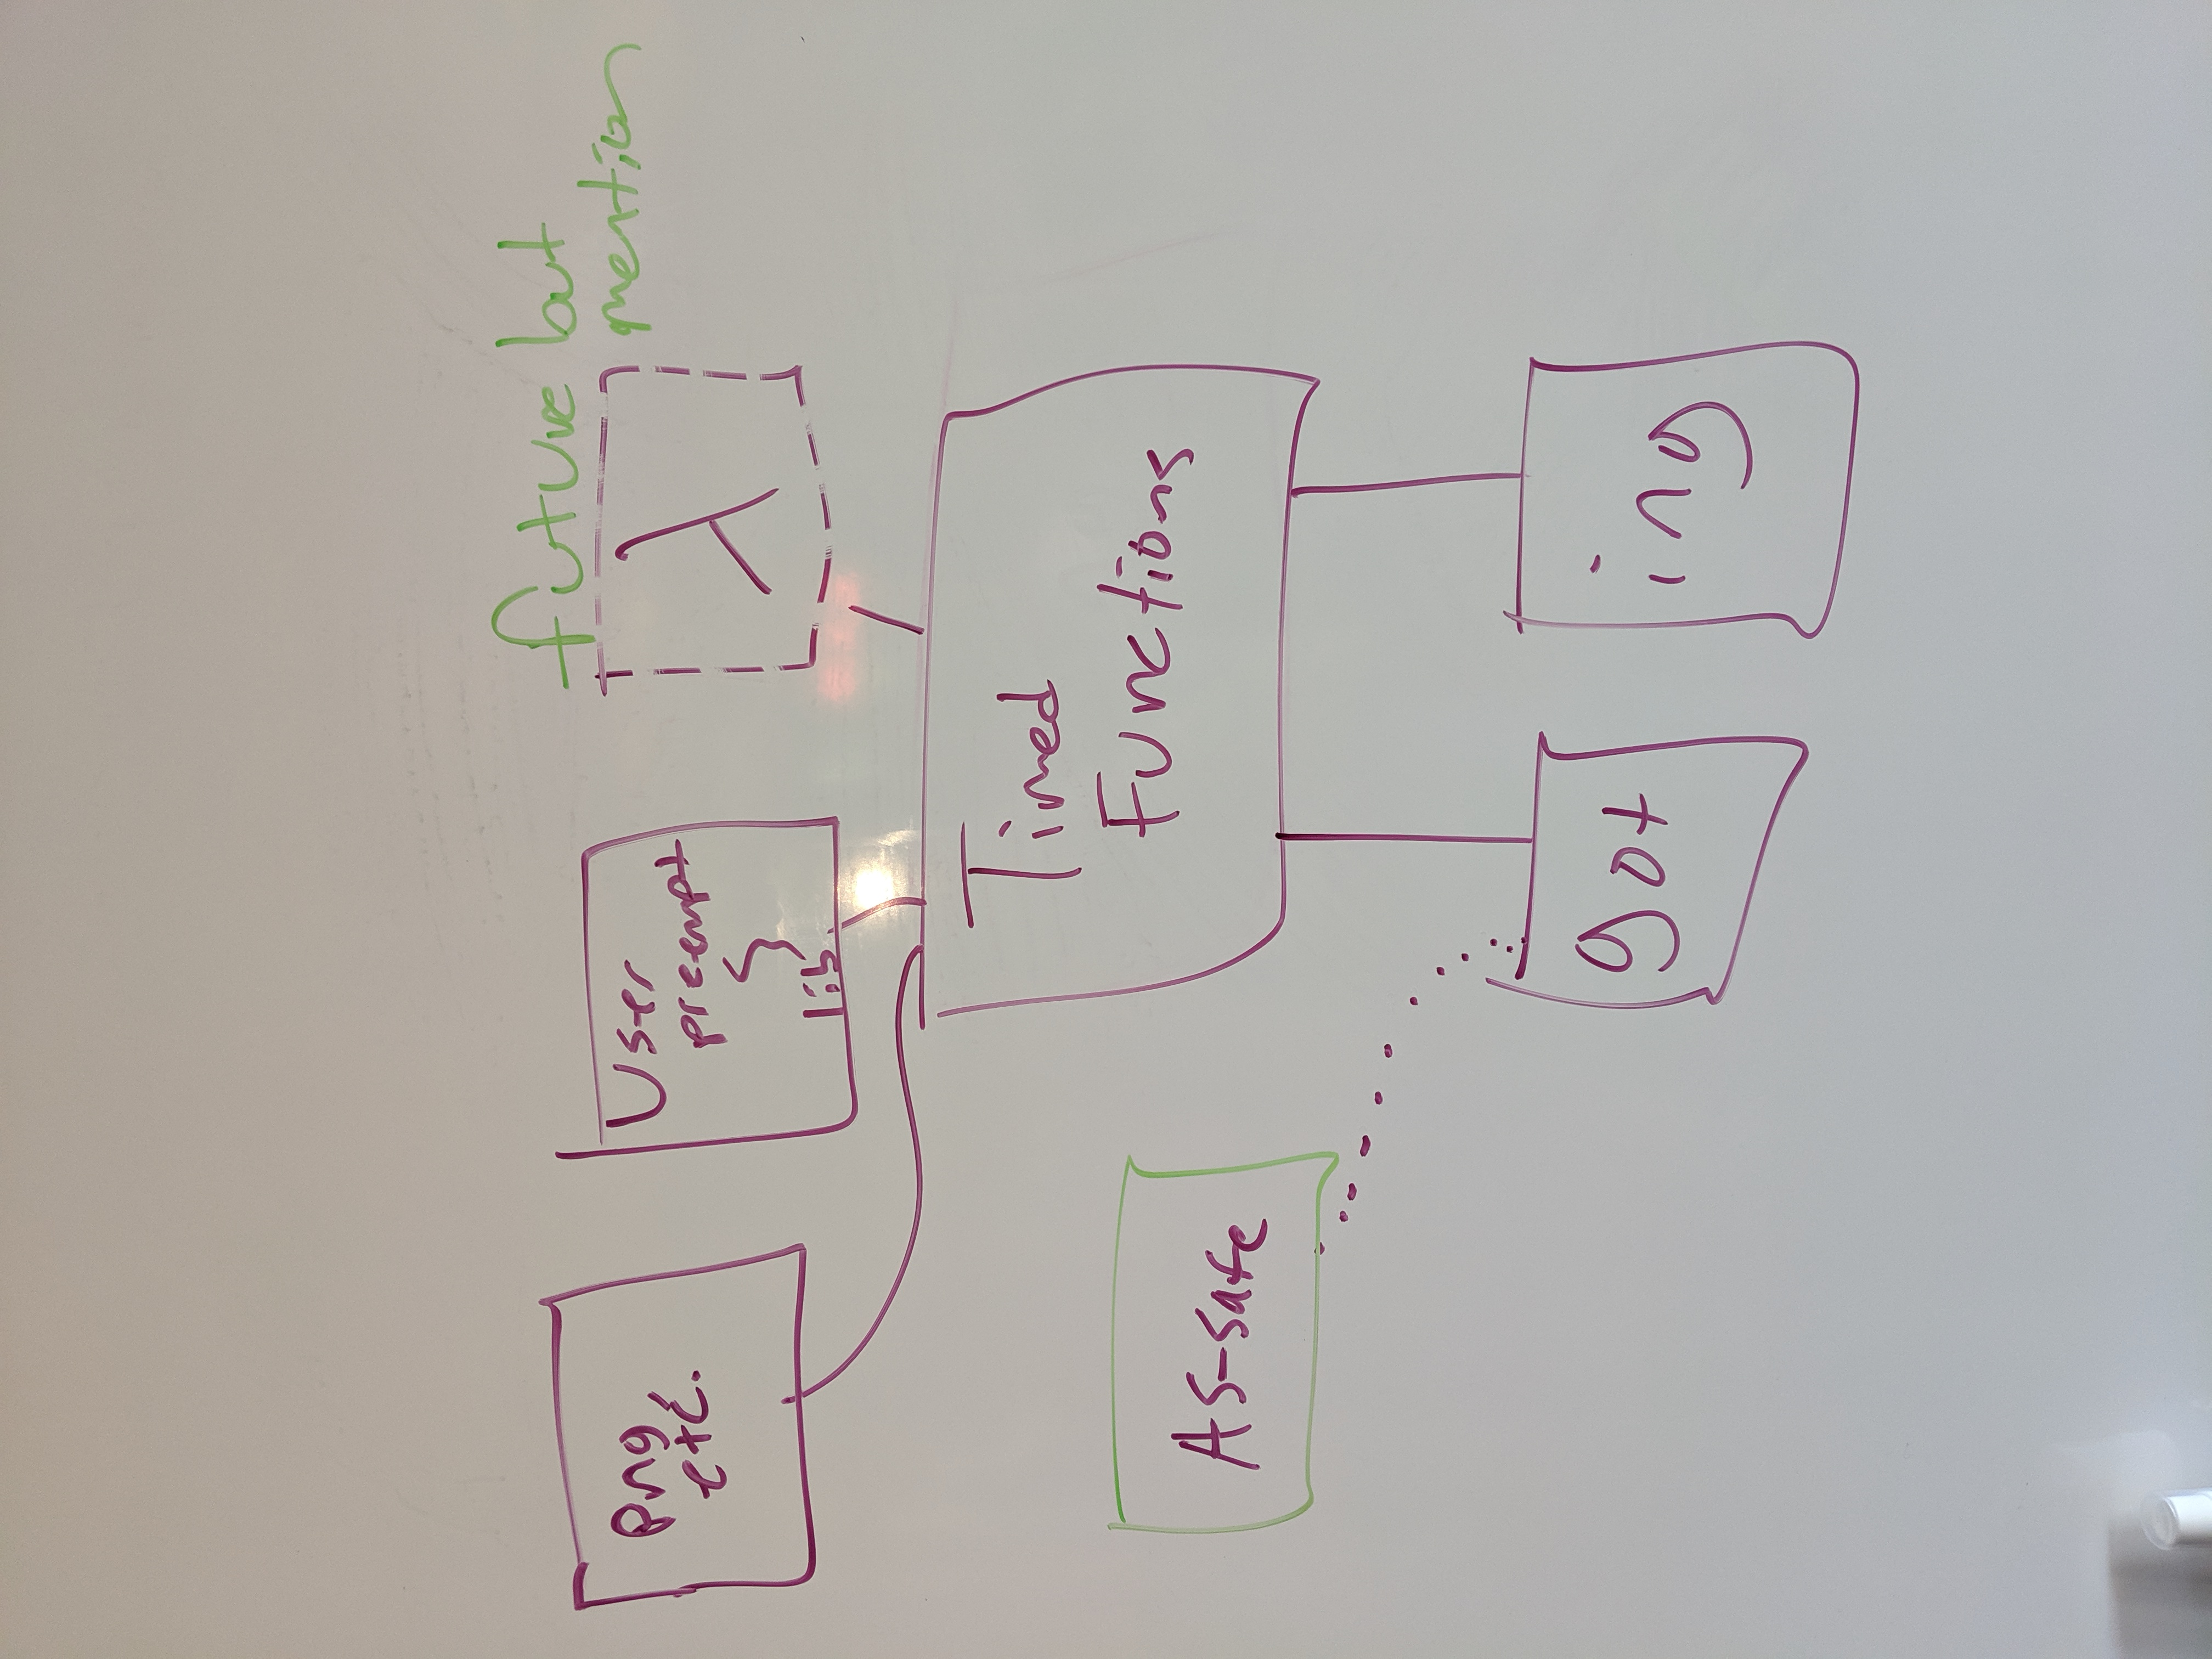
\includegraphics[width=\columnwidth]{figs/architecture}
\end{center}
\caption{Preemptible functions software stack.  \textnormal{Hexagonal boxes show
the required runtime environment.  Rectangular boxes represent components
implementing the preemptible functions abstraction.  Ovals represent components built
on top of these.  A preemptible function's body (i.e., \texttt{func}) may be defined
directly in
your program, or in some other loaded library.}}
\label{fig:architecture}
\end{figure}

\thesis{Give a tour of \textit{libtimetravel}?}
